%% Hjort & Poulsen (2019, AER) 発表スライド
%% コンパイル: lualatex hjort_poulsen_slides.tex（2回）
\documentclass[aspectratio=169,11pt]{beamer}

%% ---- 日本語 ----
\usepackage{luatexja}っっっっっk
\usepackage[haranoaji]{luatexja-preset}
\renewcommand{\kanjifamilydefault}{\gtdefault}

%% ---- パッケージ ----
\usepackage{amsmath,amssymb}
\usepackage{booktabs}
\usepackage{tikz}
\usetikzlibrary{arrows.meta,positioning,calc}

%% ---- 見た目 ----
\definecolor{navy}{HTML}{1F3864}
\definecolor{accent}{HTML}{C0392B}
\definecolor{okgreen}{HTML}{2E7D32}
\definecolor{softgray}{HTML}{F2F4F8}
\setbeamercolor{frametitle}{fg=navy}
\setbeamercolor{title}{fg=navy}
\setbeamercolor{structure}{fg=navy}
\setbeamercolor{block title}{bg=navy,fg=white}
\setbeamercolor{block body}{bg=softgray}
\setbeamercolor{block title alerted}{bg=accent,fg=white}
\setbeamercolor{block body alerted}{bg=softgray}
\setbeamercolor{alerted text}{fg=accent}
\setbeamertemplate{navigation symbols}{}
\setbeamertemplate{itemize items}[circle]
\setbeamertemplate{blocks}[rounded]
\setbeamerfont{frametitle}{size=\Large,series=\bfseries}
\setbeamertemplate{footline}{%
  \hfill{\scriptsize\color{gray}\insertframenumber\,/\,\inserttotalframenumber}\hspace{1.2em}\vspace{0.8em}}

%% 論文の図を貼る場所（\includegraphics に差し替える）
\newcommand{\figbox}[3]{%
  \begin{tikzpicture}
    \draw[gray,dashed,rounded corners] (0,0) rectangle (#1,#2);
    \node[gray,align=center,font=\small] at (#1/2,#2/2) {#3};
  \end{tikzpicture}}
\newcommand{\pp}{\,\%pt}
\newcommand{\src}[1]{\par\vfill{\scriptsize\color{gray}#1}}

\title{The Arrival of Fast Internet and Employment in Africa}
\subtitle{Hjort \& Poulsen (2019, \textit{American Economic Review})}
\author{村田 匠}
\institute{因果推論 発表}
\date{2026年11月}

\begin{document}

%% =========================================================
\begin{frame}
  \titlepage
\end{frame}

%% =========================================================
%% 1. 問い
\begin{frame}{問い：発展途上国で格差を広げたICTは、途上国でも同じか}
  \begin{itemize}
    \item 先進国では、コンピュータやブロードバンドが\alert{高技能者に有利}に働き、賃金・雇用格差を広げた（技能偏向的技術変化, SBTC）
    \item 途上国でICTがどう効くかの\alert{因果的な証拠はない}
    \begin{itemize}
      \item ICTは「儲かりそうな場所」に導入される $\Rightarrow$ 単純比較では因果効果が分からない
    \end{itemize}
  \end{itemize}
  \vspace{0.6em}
  \begin{block}{本論文の問い}
    アフリカ12か国で、高速インターネットの到来は\\
    \textbf{(1) 雇用を増やすか}　\textbf{(2) 誰の雇用を増やすか}
  \end{block}
  \vspace{0.4em}
  \textbf{答え}：就業確率は 2.2〜7.7\pp 上昇。低学歴層も含めて増え、格差はむしろ縮小
\end{frame}

%% =========================================================
%% 2. 単純比較の問題とDAG
\begin{frame}{単純比較の問題：幹線は経済的に有望な場所に敷かれる}
  \begin{columns}[T]
    \begin{column}{0.48\textwidth}
      \centering
      \begin{tikzpicture}[
          node distance=1.2cm and 1.6cm,
          v/.style={draw,rounded corners,fill=softgray,align=center,font=\small,minimum height=2.2em},
          u/.style={draw,dashed,rounded corners,align=center,font=\small,minimum height=2.2em},
          >={Stealth[length=2mm]}]
        \node[v] (D) {幹線への近さ\\（Connected）};
        \node[v, right=of D] (Y) {雇用};
        \node[u, above=1.0cm of $(D)!0.5!(Y)$] (U1) {時間不変の交絡\\（都市規模・立地）};
        \node[u, below=1.0cm of $(D)!0.5!(Y)$] (U2) {時間変化する交絡\\（道路・電力網の整備）};
        \draw[->,thick] (D) -- node[above,font=\scriptsize]{?} (Y);
        \draw[->] (U1) -- (D); \draw[->] (U1) -- (Y);
        \draw[->] (U2) -- (D); \draw[->] (U2) -- (Y);
      \end{tikzpicture}
      \vspace{0.6em}
      \begin{itemize}\small
        \item 時間不変の交絡 $\to$ 固定効果で除去
        \item 時間変化する交絡 $\to$ 平行トレンドの仮定が必要
      \end{itemize}
    \end{column}
    \begin{column}{0.50\textwidth}
      \small 表1：ケーブル到着前の比較（接続 vs 非接続）\\[0.3em]
      \begin{tabular}{lrr}
        \toprule
        & 接続 & 非接続 \\
        \midrule
        就業率（DHS）       & 0.67 & 0.68 \\
        就業率（Afrobarometer） & 0.56 & 0.59 \\
        就業率（南ア QLFS）  & 0.77 & 0.71 \\
        毎日ネット利用      & 0.08 & 0.11 \\
        夜間光              & 3.62 & 1.41 \\
        \bottomrule
      \end{tabular}
      \vspace{0.5em}
      \begin{itemize}\small
        \item 南アや夜間光では水準差が大きい
        \item DiDは\alert{水準差}は問わない。問題は\alert{トレンドの差}
      \end{itemize}
    \end{column}
  \end{columns}
\end{frame}

%% =========================================================
%% 3. 研究デザイン (1/3)
\begin{frame}{研究デザイン (1)：自然実験と処置経路}
  \begin{columns}[T]
    \begin{column}{0.55\textwidth}
      \textbf{処置経路}\\[0.3em]
      \begin{tikzpicture}[
          s/.style={draw,rounded corners,fill=softgray,font=\small,minimum width=2.6cm,minimum height=1.9em,align=center},
          >={Stealth[length=2mm]}, node distance=0.35cm]
        \node[s] (a) {欧州からの海底ケーブル};
        \node[s,below=of a] (b) {沿岸の陸揚げ地点};
        \node[s,below=of b] (c) {国内の陸上バックボーン網};
        \node[s,below=of c,fill=accent!15] (d) {幹線から500m以内の地域};
        \draw[->] (a)--(b); \draw[->] (b)--(c); \draw[->] (c)--(d);
      \end{tikzpicture}
      \vspace{0.4em}
      \begin{itemize}\small
        \item コンテンツの大半は国外でホスト $\Rightarrow$ 海底ケーブルが速度に直結
        \item 国ごとに単一のバックボーン網、隣国へ波及なし\\$\Rightarrow$ \alert{国ごとに処置時点が一意}
      \end{itemize}
    \end{column}
    \begin{column}{0.43\textwidth}
      \textbf{ケーブル到着時期（図2）}\\[0.3em]
      \small
      \begin{tabular}{ll}
        \toprule
        時期 & ケーブル \\
        \midrule
        2009Q3 & Seacom, TEAMS \\
        2009Q4 & LION \\
        2010Q3 & EASSy, MainOne \\
        2011Q2 & Glo-1 \\
        2012Q2 & WACS \\
        2012Q4 & ACE \\
        \bottomrule
      \end{tabular}
      \vspace{0.5em}
      \begin{itemize}\small
        \item 到着順はケーブルの\alert{地理的な経路}で決まる
        \item 国ごとに時期がずれる $\Rightarrow$ staggered DiD
      \end{itemize}
    \end{column}
  \end{columns}
\end{frame}

%% =========================================================
%% 3. 研究デザイン (2/3)
\begin{frame}{研究デザイン (2)：推定式と推定対象}
  \textbf{推定式（式(1)）}
  \[
    y_{ijct} = \alpha + \beta\,\underbrace{\text{SubmarineCables}_{ct}\times\text{Connected}_i}_{\text{処置}}
    + \underbrace{\delta_j\times\text{Connected}_i}_{\text{約10km四方のセル}\times\text{接続}}
    + \underbrace{\gamma_{ct}}_{\text{国}\times\text{時点}} + \varepsilon_{ijct}
  \]
  \vspace{-0.5em}
  \begin{itemize}\small
    \item 処置群：幹線から500m以内　対照群：500m〜10km
    \item 国$\times$時点FEにより、比較は常に\alert{同じ国・同じ時点の中}
  \end{itemize}
  \vspace{0.3em}
  \begin{block}{処置時点とATT}
    \small
    \[
      G_i =
      \begin{cases}
        \text{国 } c(i) \text{ に最初のケーブルが届いた時点} & \text{Connected}_i = 1\\
        \infty & \text{Connected}_i = 0
      \end{cases}
    \]
    \[
      ATT(g,t) = E\bigl[\,Y_{it}(g) - Y_{it}(\infty) \mid G_i = g\,\bigr]
    \]
    $\hat\beta$ は $ATT(g,t)$ の\alert{加重平均}。重みは OLS が決める（次々ページ）
  \end{block}
\end{frame}

%% =========================================================
%% 3. 研究デザイン (3/3)
\begin{frame}{研究デザイン (3)：識別の3つの仮定と $\hat\beta$ の重み}
  \begin{columns}[T]
    \begin{column}{0.52\textwidth}
      \small
      \textbf{A1 平行トレンド}（同じ国・セル内で）
      \[
        E[\Delta Y_t(\infty)\mid G=g] = E[\Delta Y_t(\infty)\mid G=\infty]
      \]
      \textbf{A2 予測欠如}
      \[
        Y_{it}(g) = Y_{it}(\infty)\quad (t < g)
      \]
      \textbf{A3 SUTVA（無波及）}\\
      非接続地域の潜在結果は、接続地域の処置に依存しない
      \vspace{0.3em}
      \begin{itemize}
        \item A1 $\to$ スライド「平行トレンド」
        \item A2, A3 $\to$ スライド「予測欠如とSUTVA」
      \end{itemize}
    \end{column}
    \begin{column}{0.46\textwidth}
      \small
      \textbf{$\hat\beta$ の重み}
      \[
        \hat\beta \;\approx\; \sum_c w_c\,\hat\beta_c
      \]
      \[
        w_c \;\propto\; N_c\,p_c(1-p_c)\,q_c(1-q_c)
      \]
      \begin{itemize}
        \item $p_c$：接続地域の割合、$q_c$：到着後の期の割合
        \item 国内では対照が\alert{一度も処置されない}\\$\Rightarrow$ $w_c \ge 0$（禁じられた比較なし）
        \item ただし\alert{単純平均ではない}\\観測が多く、接続・非接続が半々の国ほど重い
      \end{itemize}
    \end{column}
  \end{columns}
  \src{重みの式は均衡パネルでの近似（積み重ねたDiD：Wing, Freedman \& Hollingsworth 2024）}
\end{frame}

%% =========================================================
%% 4. 第1段階とITT
\begin{frame}{第1段階とITT：ケーブルで速度と利用が増えた}
  \small 表2：$\text{SubmarineCables}\times\text{Connected}$ の係数\\[0.3em]
  \centering
  \begin{tabular}{lccc}
    \toprule
    被説明変数 & 基本 & Connected$\times$時点FE & 平均 \\
    \midrule
    ネット速度（asinh, Akamai） & 0.362 (0.176) & 0.380 (0.191) & --- \\
    毎日利用（0/1, Afrobarometer）& 0.082 (0.028) & 0.124 (0.050) & 0.10 \\
    毎週利用（0/1, Afrobarometer）& 0.123 (0.032) & 0.142 (0.053) & 0.20 \\
    \bottomrule
  \end{tabular}
  \raggedright
  \vspace{0.6em}
  \begin{itemize}
    \item 速度は約36\%上昇（測定方法上、\alert{過小推定}：脚注37）
    \item 毎日利用は +8.2\pp（平均0.10に対して約8割増）。本文の「8 percent」は\%ptの意味
    \item 価格低下も経路の一つ：到着後にブロードバンド料金が下落（付録図A1）
  \end{itemize}
  \begin{alertblock}{解釈}
    $\hat\beta$ は「ネットを使った効果」ではなく\textbf{利用可能になったことの効果（ITT）}。\\
    IVで利用の効果を推定してはいない
  \end{alertblock}
\end{frame}

%% =========================================================
%% 5. 主結果
\begin{frame}{主結果：就業確率は 2.2〜7.7\%pt 上昇}
  \small 表3 パネルA：被説明変数＝就業（0/1）\\[0.3em]
  \centering
  \begin{tabular}{lccc}
    \toprule
    & DHS（8か国） & Afrobarometer（9か国） & 南ア QLFS \\
    \midrule
    $\hat\beta$ & 0.046 (0.014) & 0.077 (0.037) & 0.022 (0.008) \\
    平均 & 0.68 & 0.58 & 0.72 \\
    相対効果 & +6.9\% & +13.2\% & +3.1\% \\
    観測数 & 59,914 & 7,918 & 280,641 \\
    \bottomrule
  \end{tabular}
  \raggedright
  \vspace{0.6em}
  \begin{columns}[T]
    \begin{column}{0.5\textwidth}
      \textbf{本物の雇用増か？（南ア, パネルB）}
      \begin{itemize}\small
        \item 労働時間 +約10\% $\to$ 仕事の細切れ化ではない
        \item フォーマル +1.7\pp、インフォーマル +0.4\pp（n.s.）\\$\to$ 単なるフォーマル化ではない
        \item $0.017 + 0.004 \approx 0.022$（全体）
      \end{itemize}
    \end{column}
    \begin{column}{0.48\textwidth}
      \textbf{注意}
      \begin{itemize}\small
        \item 「就業」の定義・対象年齢がデータごとに違う
        \item Afrobarometer は精度が低い（95\%CI：約0.4〜15\pp）
        \item 南アは到着後が約4四半期のみ
      \end{itemize}
    \end{column}
  \end{columns}
\end{frame}

%% =========================================================
%% 6. 平行トレンド (1/2)
\begin{frame}{平行トレンド (1)：論文が示した証拠}
  \begin{columns}[T]
    \begin{column}{0.48\textwidth}
      \centering
      %% 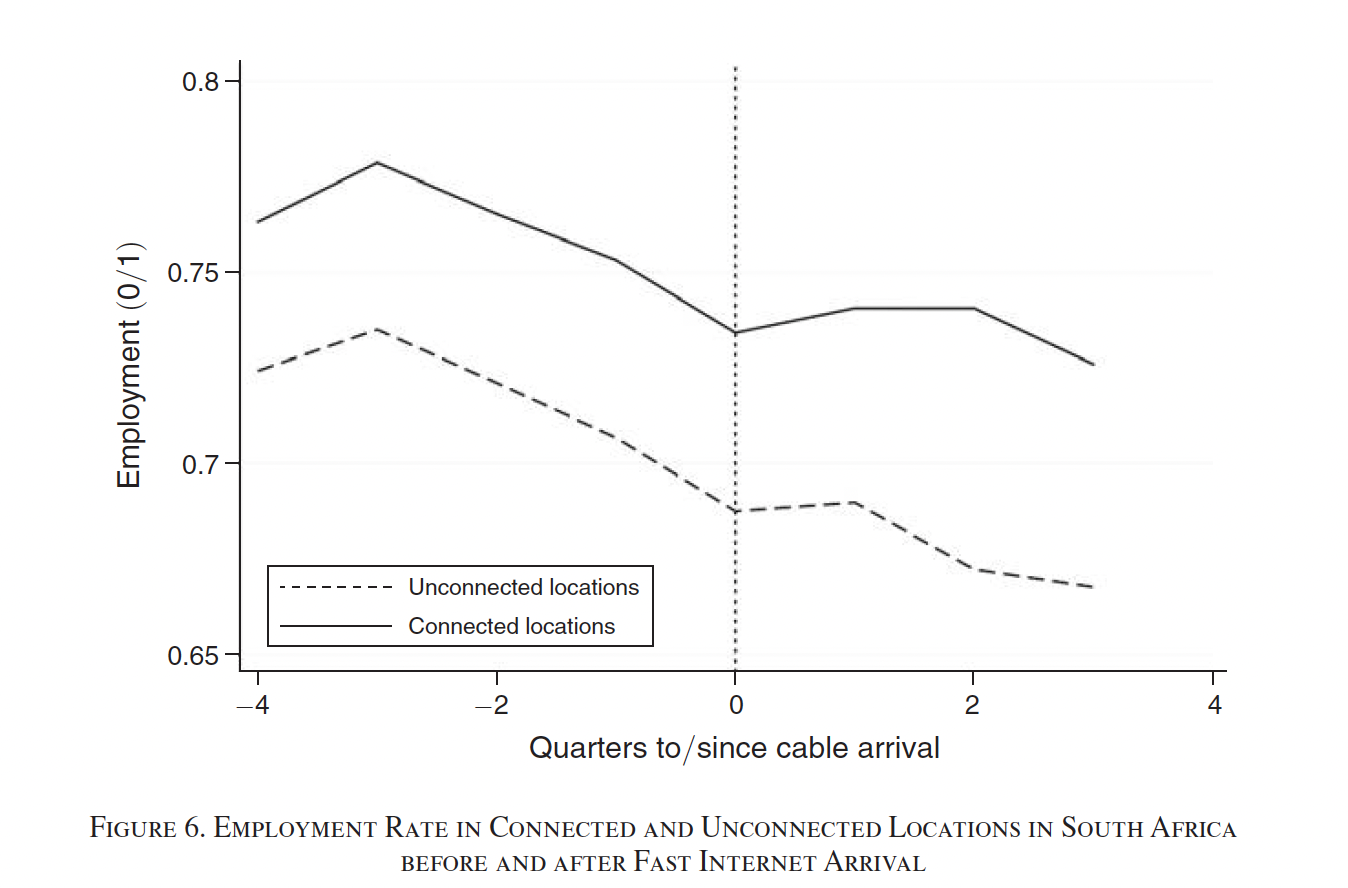
\includegraphics[width=\linewidth]{fig6.png}
      \figbox{6.0}{4.2}{図6を貼る\\南ア：接続・非接続地域の就業率\\（到着前後 $\pm$4四半期）}
      \raggedright
      \begin{itemize}\small
        \item 到着前は2本の線の\alert{形}がほぼ同じ
        \item 両方の低下は金融危機（共通ショック）
        \item 到着後に差が開いていく
      \end{itemize}
    \end{column}
    \begin{column}{0.50\textwidth}
      \small 表4：頑健性（被説明変数＝就業）\\[0.3em]
      \begin{tabular}{lc}
        \toprule
        追加した項 & 係数 \\
        \midrule
        先行項 $t+1$（南ア） & 0.005 (0.007) \\
        遅行項 $t-1$（南ア） & 0.000 (0.008) \\
        プラセボ：道路（DHS） & $-0.014$ (0.009) \\
        プラセボ：電力網（DHS） & 0.006 (0.009) \\
        プラセボ：3G（南ア） & 0.007 (0.006) \\
        セル別線形トレンド（南ア） & 0.017 (0.010) \\
        \bottomrule
      \end{tabular}
      \vspace{0.4em}
      \begin{itemize}\small
        \item 先行項ほぼゼロ $\to$ 事前トレンドなし
        \item 道路・電力網と並走していても、それらの効果ではない
      \end{itemize}
    \end{column}
  \end{columns}
\end{frame}

%% =========================================================
%% 6. 平行トレンド (2/2)
\begin{frame}{平行トレンド (2)：事前検定の限界と追加でできること}
  \begin{alertblock}{検証できる範囲が狭い}
    \begin{itemize}
      \item 事前トレンドを見られるのは\alert{南アのみ}（先行項は1期だけ）
      \item DHS・Afrobarometer は到着前の観測が1回程度 $\Rightarrow$ 図6のような確認ができない
    \end{itemize}
  \end{alertblock}
  \vspace{0.4em}
  \begin{columns}[T]
    \begin{column}{0.32\textwidth}
      \textbf{事前検定の限界}\\[0.2em]
      \small Roth (2022)\\
      検定を通過したことに頼ると、推定にバイアスが残りうる。検出力も低い
    \end{column}
    \begin{column}{0.32\textwidth}
      \textbf{感度解析}\\[0.2em]
      \small Rambachan \& Roth (2023)\\
      平行トレンドからのずれを許したとき、結論はどこまで保たれるか $\to$ \alert{本論文では未実施}
    \end{column}
    \begin{column}{0.32\textwidth}
      \textbf{変数変換}\\[0.2em]
      \small Roth \& Sant'Anna (2023)\\
      平行トレンドは尺度に依存。労働時間・企業参入は asinh 変換。主結果の就業は 0/1 なので影響なし
    \end{column}
  \end{columns}
\end{frame}

%% =========================================================
%% 7. 予測欠如とSUTVA (1/2)
\begin{frame}{予測欠如：ケーブル敷設は事前に分かっていたのでは？}
  \begin{columns}[T]
    \begin{column}{0.5\textwidth}
      \textbf{崩れるとどうなるか}
      \begin{itemize}\small
        \item 到着を見込んで、幹線沿いで先に企業参入・採用
        \item DiDが識別するのは ATT $-$（予測効果）
        \item 予測効果は同じ符号 $\Rightarrow$ \alert{過小推定}の方向
      \end{itemize}
      \vspace{0.4em}
      \textbf{論文の対応}（「予測欠如」としての明示的議論はない）
      \begin{itemize}\small
        \item 先行項 $t+1$ がほぼゼロ（南ア）
        \item 陸揚げ地点から20km以内を除いても不変（表A2）\\$\to$ 建設需要そのものの効果ではない
        \item \alert{到着前（2009年）の網}で処置群を定義\\$\to$ 見込みで新設された区間は含まない
      \end{itemize}
    \end{column}
    \begin{column}{0.47\textwidth}
      \begin{alertblock}{弱い点}
        \small
        \begin{itemize}
          \item 先行項は1期のみ。数四半期前からの予測は捉えられない
          \item 多国データでは検証不可能
        \end{itemize}
      \end{alertblock}
      \vspace{0.4em}
      \begin{block}{改善案}
        \small
        Malani \& Reif (2015) のように、ケーブル計画の\textbf{公表時点}を基準にした分析
      \end{block}
    \end{column}
  \end{columns}
\end{frame}

%% =========================================================
%% 7. 予測欠如とSUTVA (2/2)
\begin{frame}{SUTVAと処置の定義：雇用は移っただけでは？}
  \begin{columns}[T]
    \begin{column}{0.48\textwidth}
      \centering
      %% 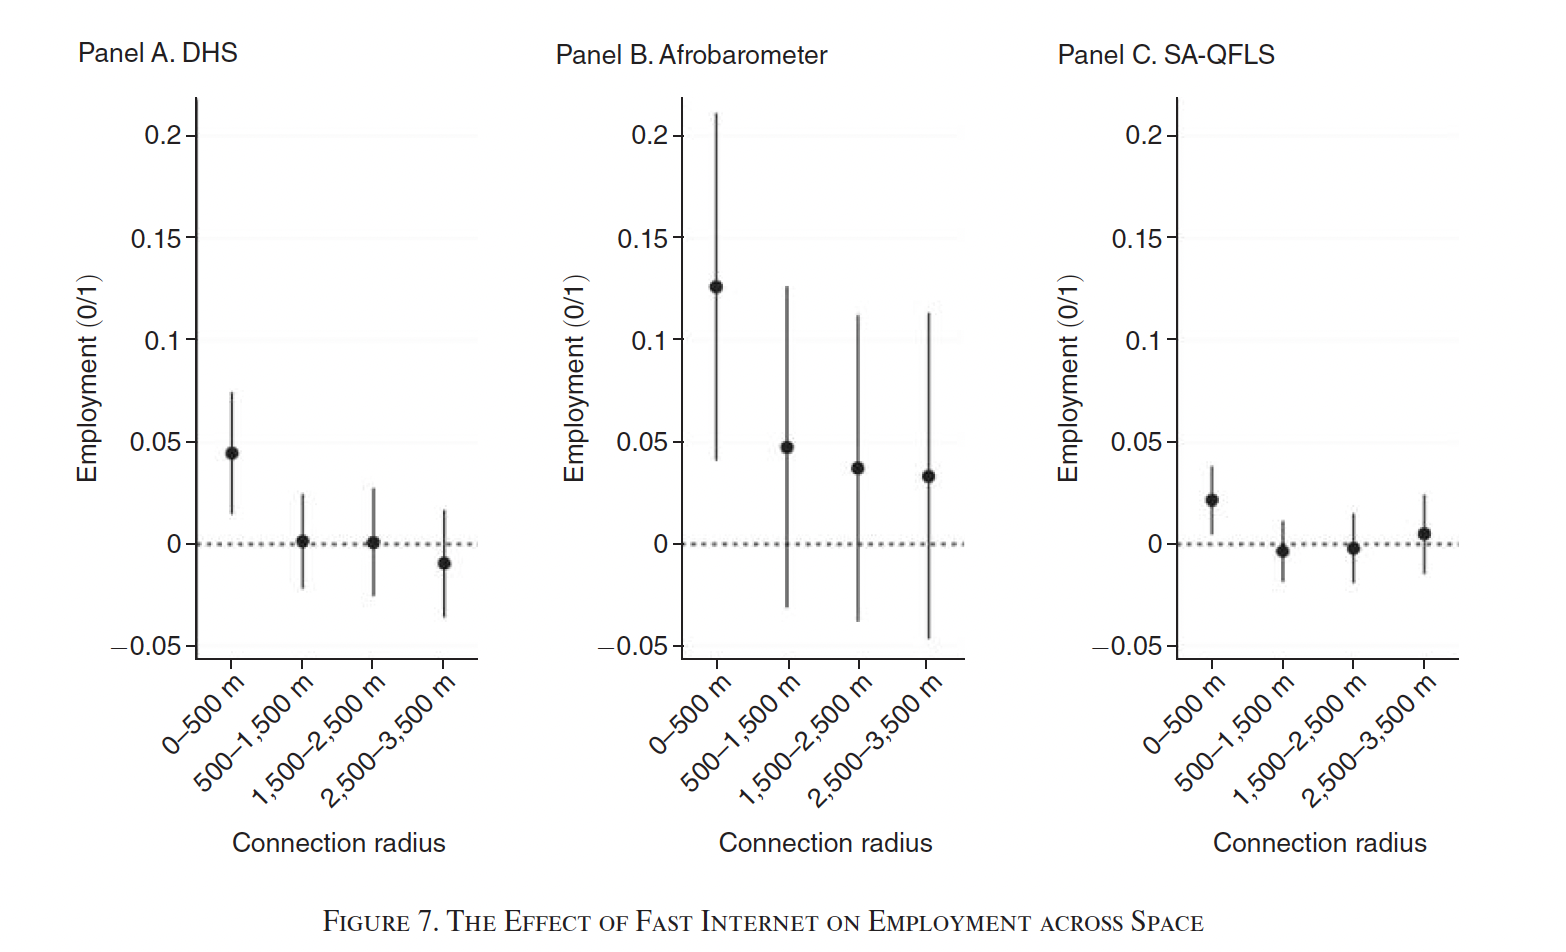
\includegraphics[width=\linewidth]{fig7.png}
      \figbox{6.0}{3.6}{図7を貼る\\距離帯別の効果\\（0--0.5 / 0.5--1.5 / 1.5--2.5 / 2.5--3.5km）}
      \raggedright
      \begin{itemize}\small
        \item 3.5km以遠を対照にし、中間の帯も別に推定
        \item 中間の帯の効果はほぼゼロ\\$\to$ 近隣から雇用を奪っていない
        \item 移住への効果もなし（南ア・タンザニア）
      \end{itemize}
    \end{column}
    \begin{column}{0.50\textwidth}
      \textbf{処置の定義（500m）}
      \begin{itemize}\small
        \item 銅線の到達距離からの保守的な線引き
        \item 半径を変えると推定値は徐々に低下（図4）\\$\to$ \alert{用量反応的}、500mの恣意的な選択ではない
        \item 対照にも弱い処置が混ざる $\to$ 効果は過小推定の方向
      \end{itemize}
      \vspace{0.4em}
      \begin{block}{評価}
        \small SUTVAへの対応は丁寧。ただし\textbf{相対効果}（接続 vs 非接続）であり、経済全体への効果ではない
      \end{block}
    \end{column}
  \end{columns}
\end{frame}

%% =========================================================
%% 8. 手法の適切さ (1/2)
\begin{frame}{手法の適切さ (1)：TWFEの重み}
  \begin{columns}[T]
    \begin{column}{0.47\textwidth}
      \textbf{主推定：安全}
      \begin{itemize}\small
        \item 国$\times$時点FE $\Rightarrow$ 比較は国内で完結
        \item 国内の対照は一度も処置されない
        \item $\dot D_{it} > 0$（処置後の接続地域）$\Rightarrow$ 負の重みなし
      \end{itemize}
      \vspace{0.4em}
      \textbf{Connected$\times$時点FEの列：要注意}
      \begin{itemize}\small
        \item 国ごとの「接続$-$非接続」の差を結果とする\alert{国レベルのstaggered TWFE}になる
        \item 一度も処置されない国はサンプルにない
        \item $\Rightarrow$ \alert{すでに処置された国}が対照に入る
      \end{itemize}
    \end{column}
    \begin{column}{0.51\textwidth}
      \small
      \textbf{例}：国A（2009年到着）、国B（2012年到着）\\[0.2em]
      \begin{tabular}{lccc}
        \toprule
        & 2008 & 2010 & 2013 \\
        \midrule
        国A & 前 & 後 & 後 \\
        国B & 前 & 前 & 後 \\
        \bottomrule
      \end{tabular}
      \[
        \textstyle\hat\beta \to ATT_A(2010) + \tfrac12 ATT_B(2013) - \tfrac12\,\alert{ATT_A(2013)}
      \]
      \begin{itemize}
        \item 効果が時間とともに増えると歪む（Goodman-Bacon 2021）
        \item 推定値は DHS 0.046$\to$0.108、Afro 0.077$\to$0.142\\\alert{「より厳しい頑健性確認」とは読めない}
      \end{itemize}
    \end{column}
  \end{columns}
\end{frame}

%% =========================================================
%% 8. 手法の適切さ (2/2)
\begin{frame}{手法の適切さ (2)：推測}
  \begin{columns}[T]
    \begin{column}{0.48\textwidth}
      \centering
      %% \includegraphics[width=\linewidth]{fig5.png}
      \figbox{6.0}{3.8}{図5を貼る\\並べ替え検定の経験分布\\（偽の到着時点を500回割り当て）}
    \end{column}
    \begin{column}{0.50\textwidth}
      \textbf{系列相関}（Bertrand, Duflo \& Mullainathan 2004）
      \begin{itemize}\small
        \item ロケーションでクラスタ
        \item 行政単位でのクラスタでも有意
        \item 並べ替え検定（南ア）：$p = 0.046$
      \end{itemize}
      \vspace{0.3em}
      \textbf{空間相関}
      \begin{itemize}\small
        \item Conley (1999) の標準誤差でも有意（表A3）
      \end{itemize}
      \vspace{0.3em}
      \begin{block}{評価}
        \small 推測への対応は十分。ただし並べ替え検定の $p$ 値は5\%をわずかに下回る程度
      \end{block}
    \end{column}
  \end{columns}
\end{frame}

%% =========================================================
%% 9. 異質性
\begin{frame}{異質性：熟練職のみ増加、教育水準別の上昇幅は同程度}
  \begin{columns}[T]
    \begin{column}{0.44\textwidth}
      \small 表5：職種別（ILO分類）\\[0.2em]
      \begin{tabular}{lcc}
        \toprule
        & 熟練職 & 非熟練職 \\
        \midrule
        DHS & 0.044 (0.018) & 0.003 (0.015) \\
        南ア & 0.014 (0.006) & $-0.001$ (0.005) \\
        \bottomrule
      \end{tabular}
      \vspace{0.4em}
      \begin{itemize}\small
        \item 雇用増は\alert{熟練職}が担う
        \item 方向は先進国のSBTCと同じ
      \end{itemize}
    \end{column}
    \begin{column}{0.54\textwidth}
      \small 表6：学歴別（被説明変数＝就業）\\[0.2em]
      \begin{tabular}{lccc}
        \toprule
        & DHS & Afrobarometer & 南ア \\
        \midrule
        初等未修了 & $-0.013$ & 0.109 & 0.012 \\
        初等修了 & 0.061 & 0.077 & 0.028 \\
        中等修了 & 0.047 & 0.060 & 0.022 \\
        高等教育 & 0.067 & 0.097 & 0.019 \\
        \bottomrule
      \end{tabular}
      \vspace{0.4em}
      \begin{itemize}\small
        \item 初等修了以上では上昇幅が\alert{同程度} $\to$ 雇用格差はむしろ縮小
        \item 熟練職の増加は高等教育層で最大（DHS 0.119）
      \end{itemize}
    \end{column}
  \end{columns}
  \src{表6は点推定のみ。標準誤差は論文を参照}
\end{frame}

%% =========================================================
%% 10. 結論と限界
\begin{frame}{結論と限界}
  \begin{block}{結論}
    \begin{itemize}
      \item 高速インターネットの到来で、接続地域の就業確率は 2.2〜7.7\pp 上昇
      \item 低学歴層も恩恵を受け、先進国のSBTCとは異なり\alert{雇用格差は拡大しない}
      \item 夜間光で測った平均所得も上昇（表9）
    \end{itemize}
  \end{block}
  \vspace{0.3em}
  \begin{columns}[T]
    \begin{column}{0.48\textwidth}
      \textbf{解釈上の注意}
      \begin{itemize}\small
        \item \alert{相対効果}：接続地域 vs 非接続地域。経済全体の効果ではない
        \item \alert{ITT}：利用可能になったことの効果
        \item $\hat\beta$ は国別ATTの分散加重平均
      \end{itemize}
    \end{column}
    \begin{column}{0.5\textwidth}
      \textbf{残る課題}
      \begin{itemize}\small
        \item 多国データでの事前トレンド・予測効果の検証
        \item 感度解析（Rambachan \& Roth 2023）
        \item 国別推定値と重みの報告、Callaway \& Sant'Anna 型の推定
      \end{itemize}
    \end{column}
  \end{columns}
\end{frame}

%% =========================================================
\begin{frame}{参考文献}
  \scriptsize
  \begin{itemize}
    \item Hjort, J. and J. Poulsen (2019). The Arrival of Fast Internet and Employment in Africa. \textit{American Economic Review}, 109(3), 1032--1079.
    \item Bertrand, M., E. Duflo and S. Mullainathan (2004). How Much Should We Trust Differences-in-Differences Estimates? \textit{QJE}.
    \item Callaway, B. and P. H. C. Sant'Anna (2021). Difference-in-Differences with Multiple Time Periods. \textit{Journal of Econometrics}.
    \item Conley, T. G. (1999). GMM Estimation with Cross Sectional Dependence. \textit{Journal of Econometrics}.
    \item de Chaisemartin, C. and X. D'Haultfœuille (2020). Two-Way Fixed Effects Estimators with Heterogeneous Treatment Effects. \textit{AER}.
    \item Goodman-Bacon, A. (2021). Difference-in-Differences with Variation in Treatment Timing. \textit{Journal of Econometrics}.
    \item Malani, A. and J. Reif (2015). Interpreting Pre-trends as Anticipation. \textit{Journal of Public Economics}.
    \item Rambachan, A. and J. Roth (2023). A More Credible Approach to Parallel Trends. \textit{Review of Economic Studies}.
    \item Roth, J. (2022). Pretest with Caution: Event-Study Estimates after Testing for Parallel Trends. \textit{AER: Insights}.
    \item Roth, J. and P. H. C. Sant'Anna (2023). When Is Parallel Trends Sensitive to Functional Form? \textit{Econometrica}.
    \item Wing, C., S. M. Freedman and A. Hollingsworth (2024). Stacked Difference-in-Differences. NBER Working Paper.
  \end{itemize}
\end{frame}

\end{document}
